\qs{}{
    What is the average family income per scholarship?
}

Calculate the average family income per scholarship by first selecting \texttt{DISTINCT} scholarship names from the \texttt{student} table. Using \texttt{AVG()}, calculate the average family income for each scholarship and present the results in descending (denoted as \texttt{DESC}) order of average family income.
\vspace{\baselineskip}

\sol{}
\noindent\line(1, 0){0.89\linewidth}
\begin{verbatim}
SELECT stud_schlr_name AS scholarship_name, AVG(stud_fam_income) AS average_family_income
FROM student
WHERE stud_schlr_name IS NOT NULL
GROUP BY stud_schlr_name
ORDER BY average_family_income DESC;
\end{verbatim}
\noindent\line(1, 0){\linewidth}

\begin{figure}[H]
    \centering
    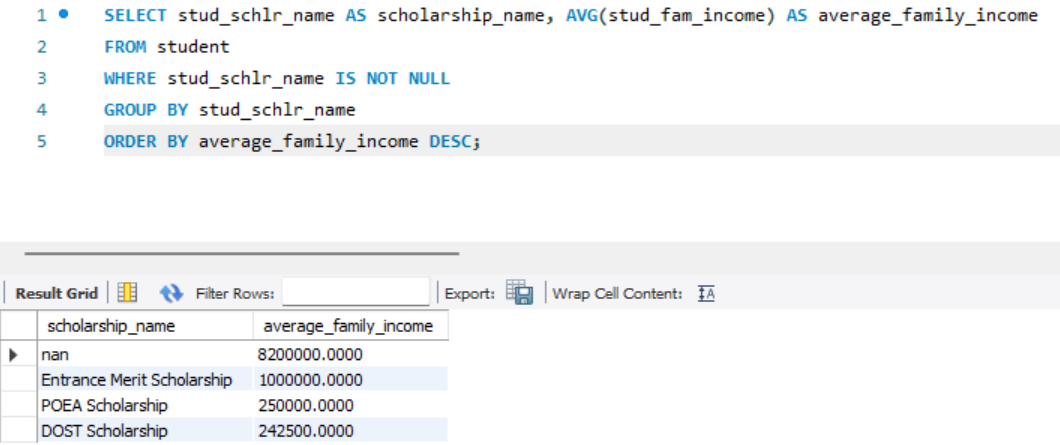
\includegraphics[width=0.7\linewidth]{images/q9.png}
    \caption{Question 9 Query and Output}
\end{figure}
